\documentclass[10pt,twocolumn]{article}

% ---------- packages (all standard; compiles on Overleaf or any TeX install) ----------
\usepackage[utf8]{inputenc}
\usepackage[T1]{fontenc}
\usepackage{amsmath,amssymb}
\usepackage{graphicx}
\usepackage{booktabs}
\usepackage[hidelinks]{hyperref}
\usepackage[margin=0.85in]{geometry}
\usepackage{caption}
\usepackage{microtype}   % better justification; fewer overfull/ragged lines
\captionsetup{font=small,labelfont=bf}

% allow long URLs / tokens to break instead of overflowing the column
\usepackage{xurl}

\graphicspath{{../figures/}}

\begin{document}

% Title + abstract span BOTH columns (full page width) for a balanced layout.
% Built from standard primitives (no \maketitle/authblk) so it is robust.
\twocolumn[{%
  \centering
  {\LARGE\bfseries Recovering a Time-Varying Transmission Rate from\\[2pt]
   COVID-19 Case Data with a Physics-Informed Neural Network\par}
  \vspace{0.8em}
  {\large Your Name\par}
  \vspace{0.3em}
  {\small Independent project. Code and data:
   \url{https://github.com/your-username/epidemic-pinn}\par}
  \vspace{1.4em}
  \begin{minipage}{0.86\textwidth}
  \begin{center}\textbf{Abstract}\end{center}
\noindent
The transmission rate $\beta(t)$ of an epidemic, and the reproduction number
$R_0(t)=\beta(t)/\gamma$ derived from it, is the single quantity public-health
teams most want to track, yet it cannot be measured directly. We treat its
reconstruction as an \emph{inverse problem}: given only a noisy, scaled proxy of
one compartment (reported daily cases), recover the hidden, time-varying
$\beta(t)$ that, when fed through a mechanistic SEIR model, reproduces the data.
We represent $\beta(t)$ as a small neural network of time and train it by
backpropagating a data-fit loss \emph{through a differentiable SEIR ODE
integrator}, so the epidemiological dynamics are satisfied exactly by
construction. On synthetic data with a known $\beta(t)$ the method recovers it to
$2.6\%$ relative-$L_2$ error (5\% noise), degrading gracefully to $3.8\%$ at
$20\%$ noise and $4.0\%$ with only biweekly observations. On Germany's first
COVID-19 wave it recovers an effective reproduction number $R_{\mathrm{eff}}(t)$
that matches Our World in Data's \emph{independent} estimate to RMSE $0.14$,
placing the epidemic turning point ($R=1$) on 8~April~2020, about two weeks after
the national lockdown. It outperforms a classical growth-rate estimator by
$\sim\!10\times$. We are explicit about the central limitation: $\beta(t)$ is
identifiable only where infectious prevalence is non-negligible, and its absolute
level is confounded with the (fixed) reporting fraction.
  \end{minipage}
  \vspace{1.5em}
}]

% =====================================================================
\section{Introduction}
% =====================================================================
During an epidemic, the most important number for decision-making is the
\emph{reproduction number}: how many further infections each infected person
causes. When it exceeds one, the epidemic grows; when it drops below one, it
recedes. It is governed by the \emph{transmission rate} $\beta(t)$, which changes
over time as behaviour and policy change (lockdowns, distancing, reopening). The
difficulty is that $\beta(t)$ is never observed. What we observe is a noisy,
incomplete count of \emph{reported cases}, a scaled and delayed shadow of the true
infection process.

Recovering an unobserved cause from its observed effect is an \emph{inverse
problem}. Inverse problems are typically ill-posed: many different $\beta(t)$
trajectories can produce similar-looking case curves, so naive curve-fitting
overfits noise and yields physically meaningless answers. The standard remedy is
to constrain the solution with a \emph{mechanistic model} of the dynamics, here
a compartmental epidemic model. This is exactly the setting of
\emph{physics-informed neural networks} (PINNs)~\cite{raissi2019}, which fit data
while enforcing a governing differential equation.

This project makes one focused contribution. Classical PINN inverse problems
recover a \emph{single constant} unknown parameter~\cite{shaier2021}; a real
epidemic needs a \emph{free function} $\beta(t)$ that rises and falls over months.
Following the line of work in~\cite{kharazmi2021,millevoi2023,long2021}, we
represent $\beta(t)$ as a dedicated small neural network. Crucially, rather than
the usual ``soft'' PINN that penalises the ODE residual at scattered points (which
we found unstable on real low-prevalence data, \S\ref{sec:method}), we train the
network \emph{through a differentiable numerical integrator} of the SEIR system.
The physics is then satisfied \emph{exactly}, there are no competing loss terms to
balance, and recovery becomes robust. This is a neural-ODE
formulation~\cite{chen2018} specialised to epidemic inverse problems.

% =====================================================================
\section{Background: the SEIR model and the inverse problem}
% =====================================================================
\paragraph{The compartmental model.}
The SEIR model~\cite{kermack1927} divides a population of size $N$ into four
fractions that sum to one: \textbf{S}usceptible (can be infected),
\textbf{E}xposed (infected but not yet infectious; the latent/incubation stage),
\textbf{I}nfectious (can transmit), and \textbf{R}ecovered (immune). People flow
$S\to E\to I\to R$ according to
%
\begin{align}
\frac{dS}{dt} &= -\,\beta(t)\,S\,I, \label{eq:S}\\
\frac{dE}{dt} &= +\,\beta(t)\,S\,I - \sigma E, \label{eq:E}\\
\frac{dI}{dt} &= +\,\sigma E - \gamma I, \label{eq:I}\\
\frac{dR}{dt} &= +\,\gamma I. \label{eq:R}
\end{align}
%
Here $\beta(t)$ is the per-day transmission rate (the unknown we recover);
$\sigma$ is the rate of leaving the latent stage ($1/\sigma$ is the mean
incubation period); and $\gamma$ is the recovery rate ($1/\gamma$ is the mean
infectious period). The nonlinear term $\beta\, S\, I$ encodes that new infections
require contact between a susceptible and an infectious person.

\paragraph{The quantities we report.}
The basic reproduction number is $R_0(t)=\beta(t)/\gamma$, and the
\emph{effective} reproduction number, which accounts for the shrinking
susceptible pool, is
%
\begin{equation}
R_{\mathrm{eff}}(t) = \frac{\beta(t)}{\gamma}\,S(t).
\label{eq:reff}
\end{equation}
%
$R_{\mathrm{eff}}$ is the directly interpretable curve: it crosses $1.0$ exactly
when the epidemic turns over. It is what we compare against an independent
reference estimate.

\paragraph{What we observe.}
We do not see $S,E,I,R$. We see \emph{reported new cases} per day, which we model
as the flux of people becoming symptomatic/ascertained out of the exposed
compartment, scaled by a reporting fraction $\rho\in(0,1]$:
%
\begin{equation}
\text{reported cases}(t) \;\approx\; \rho\,\sigma\, E(t)\, N.
\label{eq:obs}
\end{equation}
%
Because we observe only this one scaled signal, we must reconstruct both the full
latent state \emph{and} the free function $\beta(t)$. This is the inverse problem.

% =====================================================================
\section{Method}
\label{sec:method}
% =====================================================================
\paragraph{The transmission-rate network.}
We represent the unknown as a small multilayer perceptron $g_\phi$ of scaled time
$\tau=(t-t_0)/T\in[0,1]$, passed through a sigmoid so the output is bounded and
positive:
%
\begin{equation}
\beta(t) = \beta_{\min} + (\beta_{\max}-\beta_{\min})\,\mathrm{sigmoid}\!\big(g_\phi(\tau)\big).
\label{eq:betanet}
\end{equation}
%
The bounded output is a \emph{hard} constraint that prevents negative or exploding
transmission, and the network's small capacity acts as a smoothness prior; we add
a light penalty on $(d\beta/d\tau)^2$ to discourage fitting noise.

\paragraph{Physics by construction.}
A standard PINN would also introduce a second network for the state $(S,E,I,R)$
and penalise the ODE residual~\eqref{eq:S}--\eqref{eq:R} at scattered
``collocation'' points. We implemented this first; it proved unstable for a real
first wave, where the infected fraction is tiny ($I\!\sim\!10^{-4}$, $S\!\approx\!1$):
the state network's weakly-observed compartments drift, and the balance between
the data term and the residual term never stabilises (the recovered $R_0$
collapsed to $\approx 0$).

We instead integrate the SEIR system directly with a differentiable fourth-order
Runge--Kutta scheme driven by $\beta_\phi$, and read modelled cases off the
resulting $E(t)$ via~\eqref{eq:obs}. Because the trajectory is a genuine numerical
solution of the ODE, conservation ($S\!+\!E\!+\!I\!+\!R\!=\!1$), positivity, and
the correct coupling all hold automatically. The only unknowns are the network
$\phi$ and the two initial infected fractions $E_0,I_0$ (with $S_0=1-E_0-I_0$).
This removes the residual loss term entirely, so there is nothing to weight.

\paragraph{Loss and optimisation.}
With the physics enforced by the integrator, the objective is just a scale-free
relative data-fit term plus the smoothness prior:
%
\begin{equation}
\mathcal{L}
= \frac{\sum_k (\hat{c}_k - c_k)^2}{\sum_k c_k^2}
\;+\; \lambda \,\big\langle (d\beta/d\tau)^2 \big\rangle ,
\label{eq:loss}
\end{equation}
%
where the first term is the relative case-fit ($c_k$ are observed cases,
$\hat{c}_k$ the model's) and the second is the smoothness prior. We minimise with Adam
(global search) followed by L-BFGS (local polish). Everything runs on CPU in
double precision; one fit takes well under a minute.

\paragraph{Fixed $\sigma,\gamma$.}
Learning $\beta,\sigma,\gamma$ jointly is non-identifiable (many combinations fit
the same curve)~\cite{kharazmi2021}. We fix the infectious period $1/\gamma=5$
days ($\gamma=0.2$) and a short effective latent period $1/\sigma\approx3$ days
($\sigma=0.33$, reflecting pre-symptomatic transmission), and recover only
$\beta(t)$.

% =====================================================================
\section{Results}
% =====================================================================

% ---- Hero figure spanning both columns ----
\begin{figure*}[t]
  \centering
  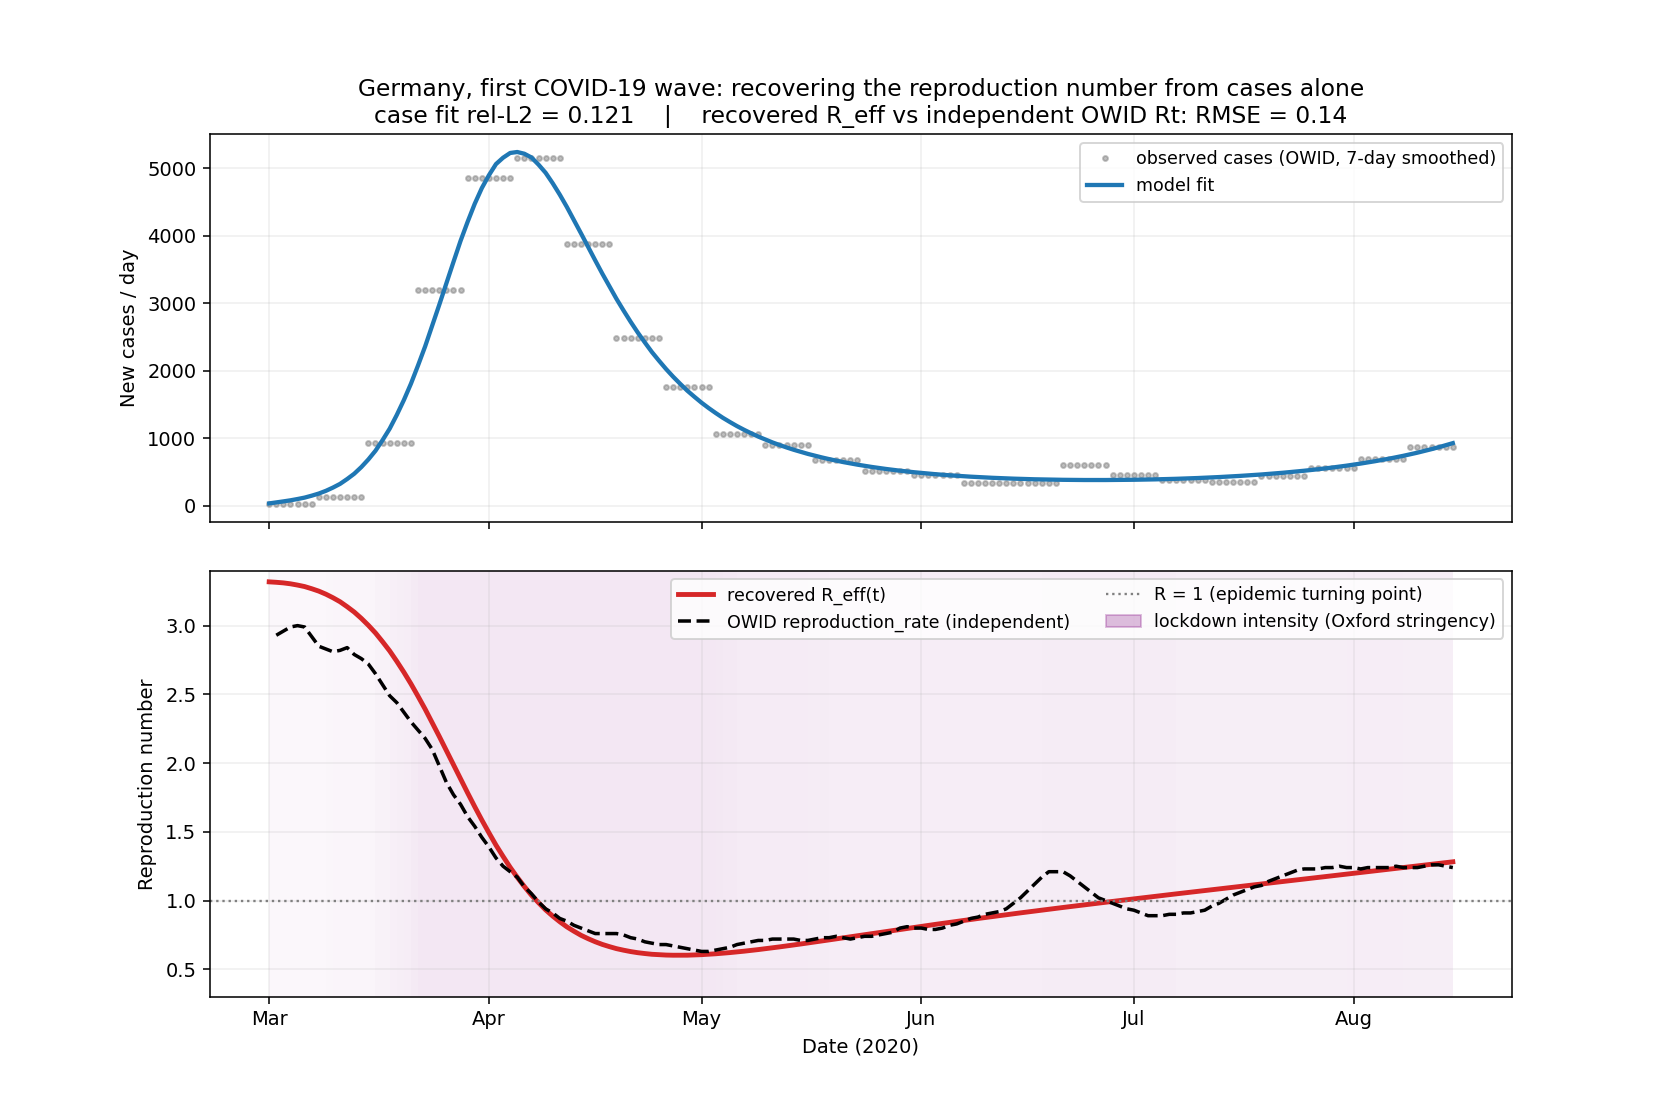
\includegraphics[width=0.92\textwidth]{headline_germany.png}
  \caption{\textbf{Headline result, Germany's first wave.} Trained only on the
  case curve (top), the model recovers an effective reproduction number
  $R_{\mathrm{eff}}(t)$ (red, bottom) that closely tracks Our World in Data's
  \emph{completely independent} reproduction-rate estimate (black dashed),
  RMSE $0.14$. It crosses the turning point $R=1$ on 8~April~2020, about two weeks
  after the national lockdown (purple shading = lockdown stringency).}
  \label{fig:hero}
\end{figure*}

\paragraph{Controlled validation (synthetic, known $\beta$).}
Before touching real data we test on data generated from a \emph{known} $\beta(t)$
(a sharp lockdown drop, $R_0: 2.5\!\to\!1.1$, during an active wave) with $5\%$
multiplicative noise. The model never sees $\beta$, only cases. It recovers
$\beta(t)$ to relative-$L_2$ error $0.026$ on the identifiable window and fits the
cases to $0.009$ (Fig.~\ref{fig:synth}). This is the proof of correctness: on real
data the true $\beta$ is unknown, so recovery can only be \emph{verified} here.

% ---- single-column synthetic figure ----
\begin{figure}[t]
  \centering
  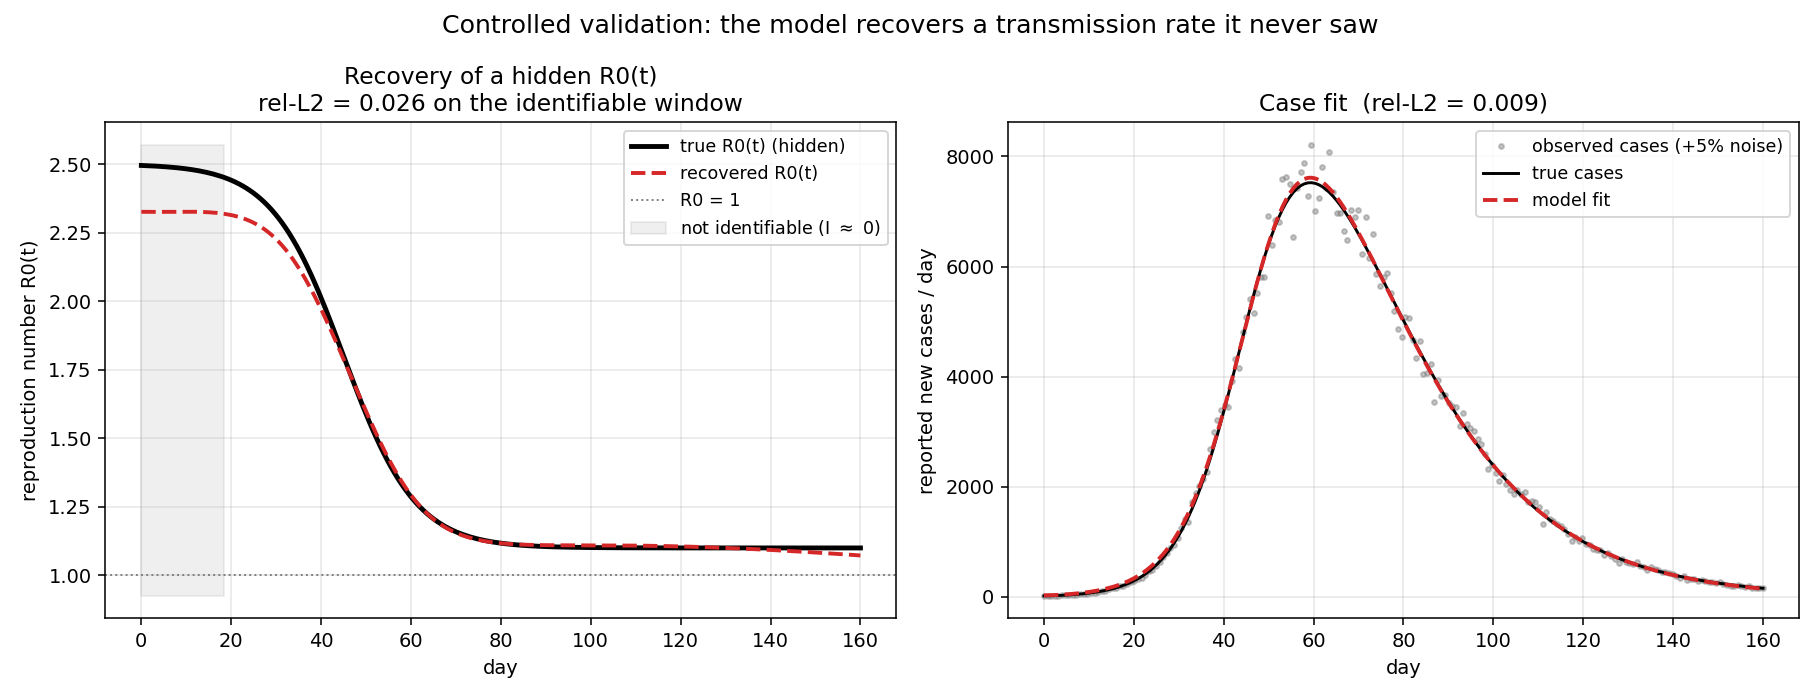
\includegraphics[width=\columnwidth]{synthetic_recovery.png}
  \caption{\textbf{Controlled validation.} The recovered $R_0(t)$ (red) tracks the
  hidden truth (black) through the whole lockdown transition. The grey band marks
  where infectious prevalence is negligible and $\beta$ is \emph{not identifiable},
  the only place the curves deviate.}
  \label{fig:synth}
\end{figure}

\paragraph{Headline: Germany's first wave (real data).}
Fitting Germany's reported cases (1~Mar--15~Aug~2020, OWID, 7-day smoothed),
Fig.~\ref{fig:hero} shows the recovered $R_{\mathrm{eff}}(t)$ against OWID's
independent reproduction-rate series. They agree to RMSE $0.14$; both fall from
$\approx 3$ through $1$ in early April and bottom out near $0.6$ in May. The
recovered level is insensitive to the reporting fraction $\rho$ (RMSE
$0.138$--$0.158$ for $\rho\in[0.05,0.20]$), consistent with the identifiability
analysis below. Key numbers are collected in Table~\ref{tab:main}.

\begin{table}[t]
\centering
\small
\setlength{\tabcolsep}{4pt}
\begin{tabular}{@{}lc@{}}
\toprule
\textbf{Quantity} & \textbf{Value}\\
\midrule
Synthetic $\beta(t)$ recovery$^\dagger$ & $0.026$\\
Synthetic case fit$^\dagger$ & $0.009$\\
Germany case fit$^\dagger$ & $0.121$\\
Germany $R_{\mathrm{eff}}$ vs.\ OWID (RMSE) & $0.144$\\
Germany recovered $R_0$ range & $[0.61,\,3.32]$\\
Germany turning point & 8 Apr 2020\\
\midrule
PINN vs.\ baseline ($R_0$)$^\dagger$ & $\mathbf{0.028}$\,/\,$0.250$\\
\bottomrule
\end{tabular}
\caption{Main quantitative results. $^\dagger$relative-$L_2$ error;
$\beta$-recovery error is on the identifiable window.}
\label{tab:main}
\end{table}

\paragraph{Robustness (synthetic, 5 seeds).}
Recovery degrades gracefully and monotonically with both noise and data sparsity
(Table~\ref{tab:robust}), the signature of a well-posed, stable method. Notably,
error barely worsens with only biweekly data (15 observations): the mechanistic
constraint compensates for missing observations.

\begin{table}[t]
\centering
\small
\begin{tabular}{@{}lccccc@{}}
\toprule
Noise & $0\%$ & $2\%$ & $5\%$ & $10\%$ & $20\%$\\
$\beta$ rel-$L_2$ & .027 & .026 & .030 & .034 & .038\\
\midrule
Interval & 1 d & 3 d & 7 d & 14 d & \\
$\beta$ rel-$L_2$ & .030 & .031 & .039 & .040 & \\
\bottomrule
\end{tabular}
\caption{Robustness to observation noise (top) and reporting interval (bottom),
mean over 5 seeds.}
\label{tab:robust}
\end{table}

\paragraph{Comparison to a classical baseline.}
A standard non-PINN approach estimates the local exponential growth rate $r(t)$ in
a sliding window and maps it to $R_0$ via the SEIR relation
$R_0=(1+r/\sigma)(1+r/\gamma)$. On the synthetic benchmark this baseline achieves
relative-$L_2$ error $0.250$ (noisy and systematically biased because it ignores
susceptible depletion and is not ODE-consistent) versus $0.028$ for our method, a
$\sim\!10\times$ improvement.

% =====================================================================
\section{Limitations}
% =====================================================================
We state these plainly, because honesty about them is part of the method's value.
\textbf{(i) Identifiability.} $\beta(t)$ is recoverable only where infectious
prevalence $I(t)$ is non-negligible; where $I\!\approx\!0$ the term $\beta S I$
vanishes and the data carry no information about $\beta$. We therefore report error
on this ``identifiable window'' and shade the rest in every figure.
\textbf{(ii) Level vs.\ shape.} With a \emph{constant} reporting fraction $\rho$,
the shape and timing of $R_0(t)$ are robust and the level only weakly sensitive to
$\rho$; a \emph{time-varying} $\rho$ (e.g.\ testing ramp-ups) would bias the level
and could masquerade as changing transmission~\cite{gostic2020}.
\textbf{(iii) Fixed $\sigma,\gamma$} are modelling choices, not measurements.
\textbf{(iv) SEIR is a simplification} (no age structure, waning immunity, or
variants). The contribution is the method, not a definitive estimate for Germany.

% =====================================================================
\section{Conclusion}
% =====================================================================
We recover a hidden, time-varying epidemic transmission rate from reported cases
by training a neural representation of $\beta(t)$ through a differentiable SEIR
integrator. The approach is validated against known ground truth, agrees with an
independent reproduction-number estimate on real data, is robust to noise and
sparse reporting, and beats a classical baseline by an order of magnitude. The
core lesson generalises beyond epidemiology: for stiff, low-signal inverse ODE
problems, \emph{integrating} the dynamics is more stable than \emph{penalising}
their residual.

% =====================================================================
\begin{thebibliography}{99}
\small

\bibitem{raissi2019} M.~Raissi, P.~Perdikaris, G.~E.~Karniadakis.
``Physics-informed neural networks: A deep learning framework for solving forward
and inverse problems involving nonlinear PDEs.''
\emph{J.\ Comput.\ Phys.} 378:686--707, 2019.

\bibitem{kermack1927} W.~O.~Kermack, A.~G.~McKendrick.
``A contribution to the mathematical theory of epidemics.''
\emph{Proc.\ R.\ Soc.\ A} 115(772):700--721, 1927.

\bibitem{kharazmi2021} E.~Kharazmi, M.~Cai, X.~Zheng, G.~Lin, G.~E.~Karniadakis.
``Identifiability and predictability of integer- and fractional-order
epidemiological models using physics-informed neural networks.''
\emph{Nature Computational Science} 1:744--753, 2021.

\bibitem{shaier2021} S.~Shaier, M.~Raissi, P.~Seshaiyer.
``Disease-Informed Neural Networks.'' arXiv:2110.05445, 2021.

\bibitem{millevoi2023} C.~Millevoi, D.~Pasetto, M.~Ferronato.
``A physics-informed neural network approach for epidemiological inverse
problems.'' arXiv:2311.09944, 2023.

\bibitem{long2021} J.~Long, A.~Q.~M.~Khaliq, K.~M.~Furati.
``Identification and prediction of time-varying parameters of COVID-19 model via
physics-informed neural networks.'' arXiv:2103.09949, 2021.

\bibitem{chen2018} R.~T.~Q.~Chen, Y.~Rubanova, J.~Bettencourt, D.~Duvenaud.
``Neural Ordinary Differential Equations.'' \emph{NeurIPS}, 2018.

\bibitem{gostic2020} K.~M.~Gostic et al.
``Practical considerations for measuring the effective reproductive number $R_t$.''
\emph{PLoS Comput.\ Biol.} 16(12):e1008409, 2020.

\bibitem{wang2021} S.~Wang, Y.~Teng, P.~Perdikaris.
``Understanding and mitigating gradient flow pathologies in physics-informed
neural networks.'' \emph{SIAM J.\ Sci.\ Comput.} 43(5):A3055--A3081, 2021.

\bibitem{hale2021} T.~Hale et al.
``A global panel database of pandemic policies (Oxford COVID-19 Government
Response Tracker).'' \emph{Nature Human Behaviour} 5:529--538, 2021.

\bibitem{arroyo2021} F.~Arroyo-Marioli, F.~Bullano, S.~Kucinskas,
C.~Rond\'on-Moreno. ``Tracking $R$ of COVID-19: A new real-time estimation using
the Kalman filter.'' \emph{PLoS ONE} 16(1):e0244474, 2021.

\bibitem{owid2020} E.~Mathieu et al.
``A global database of COVID-19 vaccinations / Our World in Data COVID-19
dataset.'' \emph{Nature Human Behaviour} 5:947--953, 2021. Data frozen 2024-08-19.

\end{thebibliography}

\end{document}
